\documentclass{report}

% ----- IMPORTS ---------------------------------------------------------------
\usepackage[ngerman]{babel}
\usepackage{float}
\usepackage[ngerman]{datetime}
\usepackage[bookmarks]{hyperref} % PDF TOC
\usepackage{graphicx}
%\usepackage{baskervald} % Use the Baskerville font
\usepackage[utf8x]{inputenc}
\setcounter{secnumdepth}{5} % include numbering in paragraph heading

% ----- META ------------------------------------------------------------------
\title{Software Engineering\\\small{WS2015/2016}}
\author{
	\textsc{Tim Bierenbreier}\\
	\normalsize Matrikel Nr.: 43235
	\and
	\textsc{Jonas Rottmann}\\
	\normalsize Matrikel Nr.: 44501
	\and
	\textsc{Jonas Weber}\\
	\normalsize Matrikel Nr.: 43399
}

% ----- CONTENT ---------------------------------------------------------------
\begin{document}

\maketitle

\tableofcontents

\chapter{Design}

\section{Aufbereitung der Analyse und Systemoperationen}
\textit{Beschreiben Sie die zu realisierenden Use Cases in Form von System-Use-Cases.
\begin{itemize}
    \item Use-Case-Beschreibung
    \item Use-Case-Diagramm
    \item detaillierte Beschreibung in Form von Activity-Diagrammen
\end{itemize}
Orientieren Sie sich hierzu an Ihren Analyseergebnissen und berücksichtigen Sie die gewählte Architektur und Ihr Bedienkonzept.}

\subsection{Use-Case-Beschreibung}
    \subsubsection{Zug spielen}
    \begin{description}
        \item[Akteure]~\par
            View, Controller
        \item[Priorität]~\par
            essentiell\\Hauptbestandteil des Spiels
        \item[Beschreibung]~\par
            \begin{itemize}
                \item [1.] Würfelzähler auf 0 zurücksetzen, Spieler der am Zug ist aus Variable auslesen und vom View ausgeben lassen.
                \item [2.] Pseudozufallszahl zwischen 1 und 6 als Würfelergebnis bestimmen, den Würfelzähler inkrementieren und Wüfelergebnis vom View anzeigen lassen.
                \item [3.] Prüfen ob der Spieler am Zug schon mindestens einen Wissensstreiter auf dem Spielfeld hat.
            \end{itemize}
            \\ Fall: Spieler am Zug hat schon mindesntens einen Wissensstreiter auf dem Feld.
            \begin{itemize}
                \item [4a.] Es sind noch nicht alle Wissensstreiter auf dem Feld und das Würfelergebnis $==$ 6, falls ja muss ein Wissensstreiter aus dem Heimatfeld auf das Startfeld gebracht werden und der Zug ist beendet.
                \item [5a.] Würfelergebnis und Positionen aller Wissensstreiter von View ausgeben lassen.
                \item [6a.] View zeigt Frage welcher Wissensstreiter bewegt werden soll an und der Controller erwartet eine Eingabe.
                \item [7a.] Eingabe wird auf Gültigkeit geprüft, man kehrt ggf. zu 6a zurück.
                \item [8a.] Die Position des Wissensstreiters wird auf die alte Position + Würfelergebnis geändert, es wird geprüft ob dieses neue Feld schon besetzt ist, und ggf. der Use-Case "`Wissen testen"' gestartet. Falls dieses Feld noch nicht besetzt ist, wird dieser Spielzug beendet.
            \end{itemize}
            \\ Fall: Spieler am Zug hat noch keine eigenen Wisssensstreiter auf dem Feld.
            \begin{itemize}
                \item [4b.] Wird geprüft ob das Wüfelergebnis $==$ 6 ist, falls ja wird ein Wissensstreiter aus dem Heimatfeld auf das Startfeld gesetzt und der Zug ist beendet. Wenn dies nicht der Fall ist wird geprüft ob der Würfelzähler $<$ 3, falls ja wird zurück zu Schritt 2. gesprungen, falls nicht ist der Spielzug ebenso beendet.
            \end{itemize}
       \item[Vorbedingungen] Spieler der am Zug ist wurde in einem Feld gespeichert.
       \item[Nachbedingung] Nächster Spieler wird im Spieler am Zug Feld vermerkt.

    \subsubsection{Wissen Testen}
    \begin{description}
        \item[Akteure]~\par
            View
        \item[Priorität]~\par
            essentiell\\Hauptbestandteil des Spiels
        \item[Beschreibung]~\par

        \begin{itemize}
            \item [1.] Präsentatiosschicht fragt den prüfenden Spieler nach einer Kategorie.
            \item [2.] Applikationssschicht wählt pseudozufällig eine Frage dieser Kategorie.
            \item [3.] Präsentationsschicht zeigt die Frage und 4 Antwortmöglichkeiten für den geprüften Spieler an und fordert Eingabe.
            \item [4.] Applikationssschicht wertet Antwort aus. Ist diese falsch wird der Wissenstandsanzeiger dekrementiert (wobei der Minimalwert 0 beträgt). Ist die Antwort richtig wird geprüft ob der Wissenstandsanzeiger schon den maximal Wert erreicht hat, ist dies der Fall fragt die Präsentationsschicht welche Kategorie ansonsten erhöht werden soll.
			\item [5.] Der Wissenstreiter des geprüften Spielers wird bewegt:
				\begin{itemize}
					\item Antwort war richtig: Wissensstreiter wird auf das Startfeld des Spielers gesetzt, ist dieses bereits besetzt muss der Wissensstreiter ins Heimatfeld.
					\item Antwort war falsch: Wissensstreiter wird zurück ins Heimatfeld gesetzt.
				\end{itemize}
			\item [6.] Die Applikation vergleicht ob der prüfende Spieler $!=$ dem geprüften Spieler, falls nicht wurde der Wissenstest beendet. Stimmen prüfender Spieler und geprüfter Spieler nicht überein fragt die Präsentationsschicht den prüfenden Spieler ob er sich selbst testen will. Falls ja geht es wieder bei Schritt 1. weiter, falls nicht ist der Wissenstest beendet.
        \end{itemize}
        \item[Vorbedingungen] Wissensstreiter wurde auf Feld gezogen, welches schon besetzt ist.
    \end{description
\end{description}

\subsection{Use-Case-Diagramm}


\subsection{Aktivitäts-Diagramme}


\subsection{System-Sequenz-Diagramme}


\subsection{System-Operationen}
\subsubsection{Zug spielen}
\paragraph{wissensstreiterBewegen (Wissensstreiter wissensstreiter)}
\begin{description}
	\item[Verantwortlichkeit] Das aktuelle Feld des vom Controller entgegengenommenen Wissensstreiters wird um die zuvor gespeicherte Augenzahl inkrementiert. Das aktuelle Feld des geschlagenen Spielers wird auf sein Heimatfeld gesetzt. Anschließend wird überprüft, ob das neue Feld leer oder belegt ist.
	\item[Bemerkungen] Gewählter Wissensstreiter wird bewegt.
	\item[Ausnahmen] keine
	\item[Vorbedingung] Spiel ist initialisiert, eine Augenzahl wurde automatisch am Anfang des Zuges generiert und ein Spieler hat eine Eingabe gemacht, welchen Wissensstreiter bewegt werden soll.
	\item[Nachbedingung] Wenn das neue Feld (altes Feld + Augenzahl) leer ist, ist der nächste Spieler am Zug. Wenn nicht, tritt der Use Case „Wissen testen“ ein.
\end{description}

\subsubsection{Wissen testen}
\paragraph{kategorieSetzen (Kategorie kategorie)}
\begin{description}
	\item[Verantwortlichkeit] Die vom Controller entgegen genommene Kategorie wird gesetzt, um daraus die folgende Frage zu entnehmen.
	\item[Bemerkungen]  Kategorie wird für Fragerunde gesetzt.
	\item[Ausnahmen] keine
	\item[Vorbedingung] Wissensstreiter wurde auf Feld gezogen, auf dem schon ein Wissensstreiter steht.
	\item[Nachbedingung] Antwort muss gewählt werden.
\end{description}

\paragraph{antwortPrüfen(int antwortNummer)}
\begin{description}
	\item[Verantwortlichkeit] Die vom Controller entgegen genommene Antwortnummer wird mit der Antwortnummer der richtigen Antwort der Frage verglichen.
	\item[Bemerkungen] Antwort wird überprüft.
	\item[Ausnahmen] keine
	\item[Vorbedingung] Eine Kategorie wurde gesetzt.
	\item[Nachbedingung] Wenn die Antwort richtig ist, wird der Wissensstandszeiger des Spielers in dieser Kategorie inkrementiert. Wenn der Wissensstandszeiger bereits den Maximalwert 3 hat, wird nochmals eine Kategorie entgegen genommen, um den Wissensstandszeiger stattdessen in dieser kategorie zu erhöhen.\newline
	Wenn die Antwort falsch ist, wird der Wissensstandszeiger dekrementiert. Wenn der befragte Spieler darüber hinaus ungleich dem fragenden Spieler ist, wird die Funktion frageBeantworten(antwortNummer) erneut für den fragenden Spieler aufgerufen.
\end{description}

\paragraph{wissensstandszeigerErhöhen(Kategorie kategorie)}
\begin{description}
	\item[Verantwortlichkeit] Der Controller nimmt eine Kategorie entgegen, in der für den aktuellen Spieler die Wissensstandszeiger-Variable inkrementiert werden soll.
	\item[Bemerkungen] keine
	\item[Ausnahmen] keine
	\item[Vorbedingung] Prüfen der Antwort lieferte true und die Wissensstandszeiger-Variable für die aktuelle Kategorie des aktuellen Spielers steht auf dem Max-Wert 3.
	\item[Nachbedingung] Nächster Spieler ist an der Reihe.
\end{description}



\section{Zustandsautomat}
\begin{figure}[H]
	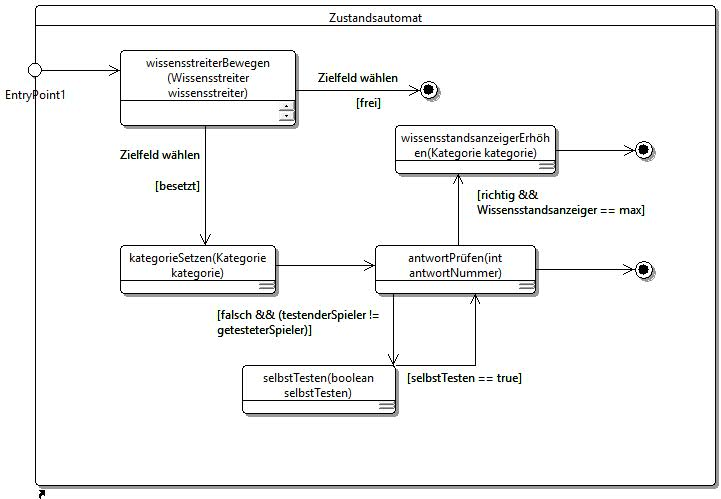
\includegraphics[width=\textwidth]{Diagramme/Zustandsautomat.jpg}
	\centering
\end{figure}

\section{Detailed Design und das Objektmodell}



\end{document}
